\section{Sampling Update Patterns}
In this section, we discuss how to efficiently sample update patterns for different types of views.
We first formalize the update patterns in Section~\ref{subsec:pattern}, and then present fast sampling techniques for them in Section~\ref{subsec:sample-pattern}. Furthermore, we also analyze the cost of our methods, and show the significant cost savings over incremental view maintenance.

\begin{figure}[t]
\centering
 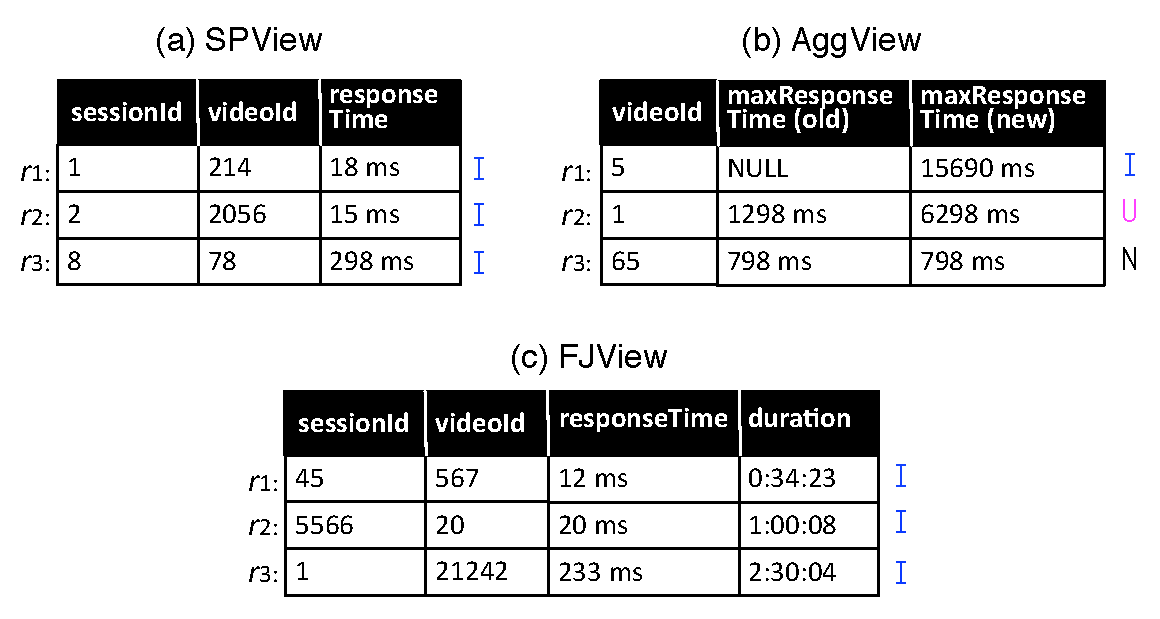
\includegraphics[scale=0.45]{figs/update-pattern.pdf}\vspace{-1em}
 \caption{Illustration of update patterns (See view definitions in Section~\ref{subsubsec:supported-view}). \reminder{Change View Def in Sec~3.1.1}}\label{fig:update-pattern}
\end{figure}


\subsection{Update Patterns}\label{subsec:pattern}
Intuitively, update patterns represent the update information involved in a stale view. With such information, we can easily transform the stale view to the corresponding up-to-date view. There are three possible update patterns. (1)~Insertion~(I): Insert a new record into a view;
(2)~Updating~(U): Update attribute values of an existing record; (3)~No Changing~(N): Keep an existing record unchanged. Figure~\ref{fig:update-pattern} illustrates the update patterns of the three types of views supported by our system.

For \spview and \fjview, the only changes of these views are inserting some new records, thus their update patterns only involve insertion.  
For example, Figure~\ref{fig:update-pattern}(a) shows that we should insert $r_1$, $r_2$ and $r_3$ into the stale \spview (See the view definition in Section~\ref{subsubsec:supported-view}). Similarly, Figure~\ref{fig:update-pattern}(c) illustrates the update patterns of the stale \fjview, which means that we should insert $r_1$ and $r_2$ into the view.

For \aggview, the changes of the view could be inserting a new group, updating the aggregation attribute values of an existing group, or keep an existing group unchanged, thus its update patterns involve insertion, updating and no changing. 
For example, Figure~\ref{fig:update-pattern}(b) illustrates the update patterns of the stale \aggview. In the figure, $r_1$ indicates that the group-by key, ``videoId = 5", does not exist in the stale view, and we need to insert this new group into the view; $r_2$ indicates that the group-by key, ``videoId = 1", is already in the stale view, and we should update the aggregation attribute value (i.e., \textsf{maxResponseTime}) of the group from 1298 ms to 6298 ms; $r_1$ indicates that the group-by key, ``videoId = 65", is already in the stale view, and we do not need to change the aggregation attribute value of the group.    



\subsection{Sampling Techniques for Update Patterns}\label{subsec:sample-pattern}
It is easy to see that getting all the update patterns for a stale view can be as expensive as incremental view maintenance. Therefore, instead of maintaining the entire update patterns, our system only maintains a random sample of the update patterns. Next we describe our sampling techniques for each type of materialized views.

\subsubsection{Select-Project and Foreign-Key Join Views}
Consider a base table $T$ and the corresponding insertion table $\triangle T$. Given a \spview defined on the table, its full update patterns involve the inserted records of $\triangle T$ that satisfy the predicate of the \spview. To sample the update patterns (e.g., at a sampling ratio of $\alpha = 5 \%$), we randomly select 5\% records from $\triangle T$, and then keep the records that satisfy the view's predicate as a sample. 

\sloppy

For a given \fjview, suppose $T$ is a fact table, and $T_1, T_2, \cdots, T_k$ are dimension tables. Its full update patterns involve the inserted records of $\triangle T \bowtie (T_1+\triangle T_1) \bowtie (T_1+\triangle T_1) \cdots \bowtie (T_k+\triangle T_k)$ that satisfy the predicate of the \fjview\footnote{Note that due to foreign constraints, it is guaranteed that the join result of $T \bowtie \triangle T_i ~(1\leq i \leq k)$ is empty}. Similar to \spview, to sample the update patterns (e.g., $\alpha= 5 \%$), we first randomly select 5\% records from $\triangle T$, and then join the selected records with new dimension tables (i.e., $\triangle T_i ~(1\leq i \leq k)$), and finally return as a sample the joined records that satisfy the view's predicate. 

\fussy


\begin{table}\renewcommand{\arraystretch}{1.2}

\caption{Cost analysis of sampling techniques for update patterns.}\label{tbl:cost-analysis}\scriptsize
%\begin{tabular}[t]{|c@{\::\:}l@{\:,\:}l@{\:,\:}r|}
\begin{tabular}[t]{|@{\:\:}l@{\:\:}||r|r|r|}
  %\multicolumn{4}{c}{\normalsize {(a) $\ars$}} \\ \hline
  %\multicolumn{4}{|c|}{A set $\Lambda$ of $\ar$s} \\ \hline\hline
   \hline
   & \spview  & \fjview & \aggview \\ \hline \hline
  Scan of Updates & $n\cdot \textrm{cost}_{read}$  & $n\cdot \textrm{cost}_{read}$ &   \\ \hline
  Delta View & $\alpha n \cdot \textrm{cost}_{pred}$  & $\alpha n \cdot \textrm{cost}_{join}$ &          \\ \hline
  Refresh    & $\alpha \delta_v \cdot \textrm{cost}_{write}$  & $\alpha \delta_v \cdot \textrm{cost}_{write}$ &  \\ \hline
\end{tabular}
\end{table}
\vspace{.5em}


{\noindent \bf Cost Analysis.} Let $n = |\triangle T|$ be the number of inserted records, $v$ be the cardinality of the stale view, $\delta_v$ be the cardinality of the full update patterns, and $\alpha$ be the sampling ratio. Table~\ref{tbl:cost-analysis} shows the cost analysis of our sampling techniques for update pattern.

\vspace{-.5em}

\begin{itemize} %[leftmargin=5.5mm]
\item Scan of Updates. Both incremental view maintenance and our proposed solution require at least one scan of the inserted records. But note that in both solutions we can load the updates into memory once and amortize that I/O cost over all views.  \vspace{-0.5em}
\item Delta View. For Select-project and foreign-key join views, incremental view maintenance has processing cost of $n$ records where the predicate or the join has to be evaluated for each inserted record. Our approach can reduce this number to $\alpha n$ as we have to evaluate this only on our sample. \vspace{-0.5em}
\item Refresh. For Select-project and foreign-key join views, incremental view maintenance has to insert $\delta_v$ rows while we have to insert only $\alpha\delta_v$ records. \reminder{Add this to ourlier indexing section? If there is an outlier index, this cost increases to $\alpha\delta_v + l$} 
\end{itemize}

From the above analysis, we can see that our sampling techniques require much less cost than incremental view maintenance for \spview and \fjview. For example, if updates have already been loaded into memory, we can save the cost of incremental view maintenance by 20 times for the sampling ratio of $\alpha = 5 \%$.

\subsubsection{Aggregation View}
The update patterns for an \aggview contains the updating information of each existing group in the view as well as newly inserted groups. Instead of maintaining the updating information for all groups, our sampling techniques only maintain such information for a sample of groups. Let $S_{V}$ denote a sample of groups in a stale \aggview.  



\iffalse
In the previous section, we discussed how the delta view did not contain enough
information to calculate a correction.
Similarly, sampling to estimate the correction for queries on Aggregation Views
is more challenging.
We notice that in the refreshed view each GROUP BY key is unique, and
thus, to sample the refreshed view we have to sample by GROUP BY keys
in the inserted records. For each inserted record we apply a hash
to the cols in the GROUP BY clause, and then we take the result of
the hash modulo a sampling ratio to sample the table. The result is
that we ensure that every record with the same group by key is either
fully in the sample or not, thus none of the rows in the delta view
are approximate. 
Then, we refresh this sample delta view instead of the full view.
We can then join this delta view with the old view to approximate $\epsilon$.

Unlike before this is not a sample of a delta view, it is a sample of the entire view joined with the stale resuts.
Thus, we denote this sample as $S_{V}$.
Also, recall that unlike the other views, Aggregation Views did not have 
an additional proportionality constant for a full correction.
\[
f(S_{V})\approx\epsilon
\]
However, when we introduce sampling a scaling constant is now neccessary.
The scaling constant $c$ for the SUM and COUNT queries depends on the sample size and is $c = \frac{K}{N}$, 
but $c = 1$ for the AVG query.
For SUM, COUNT, AVG, and VAR, this estimate of $\epsilon$ is unbiased as before.
\fi
\vspace{.5em}
{\noindent \bf Cost Analysis: }
Let $n$ be the number of inserted records, $v$ be the cardinality of the old view, $v'$ be the cardinality of the new view, $\delta_v$ be the cardinality of the delta view, and $p$ be the sampling ratio.  

\begin{itemize}
\item Scan of Updates.
As in the Select-Project and Foreign-Key Join views, both incremental maintenance and our proposed solution require at least one scan of the inserted records, and in both solutions we can load the updates into memory once and amortize that I/O cost over all views. 
\item Delta View. For aggregation views, incremental maintenance has the processing cost of $n$ and in addition an aggregation cost of $\delta_v$ where aggregates for each of the groups have to be maintained. In contrast, for aggregation views, our approach has a cost of $p\delta_v$ as we sample the group by keys and an expected processing cost of $np$. 
For aggregation views, in a distributed environment, there are potentially additional communication costs as the updates may not be partitioned by the group by key.

\item Refresh. For aggregation views, the cost is a little bit more complicated as we have a combination of insertions into the view and updates to the view. 
Incremental maintenance has to refresh $\delta_v$ rows while we have to refresh $p\delta_v$ rows. 
If there is a join index, in constant time, we can determine which rows are new insertions and which correspond to rows already in the view.

The costs become higher in a distributed environment as we need to consider communication and query processing engines that rely on partitioned joins rather than indices.
For aggregation views, we want to partition the data by the group by key.
This allows a partitioned join which only requires communication (a shuffle operation) of the delta table.
Therefore, in incremental maintenance we have to communicate $\delta_v$ rows while our solution requires $p\delta_v$ rows.
\end{itemize}










\iffalse
\section{Correction Query Processing} \label{sec:exact-correct}
To easily understand how our system works, we first simplify the design of our system by not considering sampling and ourlier indexing. We study the problem that how to \emph{exactly} correct stale query results. We formulate this problem in Section~\ref{subsec:formulation} and present a correction query processing framework to solve this problem in Section~\ref{subsec:framework}. For practical concerns, we further discuss how to implement this framework using SQL in Section~\ref{subsec:impl-sql}.

\subsection{Problem Formulation}\label{subsec:formulation}



\subsection{Correction Query Processing Framework}\label{subsec:framework}




\subsection{Implementing Correction Query Processing Using SQL}\label{subsec:impl-sql}
\fi




\iffalse

\section{Correction Query Processing}
In this section, we will describe the how to calculate a 
correction for stale queries.
Suppose we have an aggregation query $f$ and let $\textbf{V}_{T}^{'}$ be the up-to-date view
and $\textbf{V}_{T}$ be the old view. 
The query $f$ is stale with error $\epsilon$ if:
\[
f(\textbf{V}_{T}^{'})=f(\textbf{V}_{T})+\epsilon
\]
Before we discuss how sampling can scale this process, we will discuss how to correct
queries on the full data.

\subsection{Model for Aggregate Queries on Views}
What is special about SUM, COUNT, AVG, and VAR aggregate functions
is that upto proportionality constant, they can be expressed as a mean-value calculation.
For example, a SUM is just the mean value times the dataset size, a COUNT 
is the mean occurance rate times the dataset size, and VAR is mean squared 
deviation.
Let $N$ be the number of tuples in the view $V$. 
These queries can also have predicates so we have to incorporate that
as an indicator function (true = 1, false = 0) that skips a tuple in the aggregation if the predicate is false. 
When we couple these queries with predicates, we can express them in the 
following way:
\[
\forall v_i \in V \text{ : } f(V)= \frac{1}{N} \sum_i^N \phi(v_i) \cdot predicate(i)
\]

We define $\phi$ in the following way:
\begin{center}
\begin{tabular}{|c|c|}
\hline 
Aggregation Query & $\phi(v_i)$\tabularnewline
\hline 
\hline 
SUM & $N \cdot v_i$\tabularnewline
\hline 
COUNT & $N$\tabularnewline
\hline 
AVG & $\frac{N}{\sum_i^N predicate(i)} \cdot v_i$\tabularnewline
\hline 
\end{tabular}
\par\end{center}

\subsection{Corrections For Select-Project and Foreign-Key Join Views}
With the model for aggregate queries described above, we can
first derive the exact value for $\epsilon$ without sampling.
Since we only consider a model were records are inserted into the
base tables, for these two categories of views $\textbf{V}_{T}\subseteq\textbf{V}_{T}^{'}$.
The row differences between $\textbf{V}_{T}$ and $\textbf{V}_{T}^{'}$
are completely represented by the delta table $\Delta\textbf{V}$;
that is rows will only be inserted into the views. 
Since the aggregate queries are in the form of means, we notice that we 
can exploit the associativity of summations:
\[
f(\textbf{V}_{T}^{'})=f(\textbf{V}_{T})+\epsilon
\]
\[
f(\textbf{V}_{T}^{'})-f(\textbf{V}_{T})=\epsilon
\]
Upto a scaling constant c, $\epsilon$ is the aggregation function
applied to the delta table. 
\[
c\cdot f(\Delta\textbf{V})=\epsilon
\]

\begin{center}
\begin{tabular}{|c|c|}
\hline 
Aggregation Query & Scaling Constant c\tabularnewline
\hline 
\hline 
SUM & 1\tabularnewline
\hline 
COUNT & 1\tabularnewline
\hline 
AVG & $\frac{|\Delta V|}{|\Delta V|+|V|}$\tabularnewline
\hline 
\end{tabular}
\par\end{center}

\subsubsection{Example Query Processing}
Recall, our example dataset of video streaming logs and the example
selection view:
\begin{lstlisting}
View1 := SELECT * FROM Log 
WHERE userAgent 
LIKE '%Mozilla%'
\end{lstlisting}
This query filters out the log records that came from browsers with the Mozilla tag.
Let us assume that our old materialized view has 1M rows, and 
we receive an update of 500,000 new rows with the mozilla tag.
Now we want to answer the following query:
\begin{lstlisting}
SELECT avg(responseTime) 
FROM View1
\end{lstlisting}
On the inserted 500,000 rows, we can run the query and call the result $r_{delta}$.
Then, we apply the scaling constant c to the result to convert this into an $\epsilon$ and get $r_{delta}\frac{500000}{500000+1000000}$, which 
equals $\frac{r_{delta}}{3}$.
Therefore, the up-to-date result is:
\[r_{old} + \epsilon = r_{old} +\frac{r_{delta}}{3}\].

\subsection{Aggregation Views}
The delta view is not enough information to calculate $\epsilon$ in aggregation views. 
Consider the following example view which we described in the last section:
\begin{lstlisting}
View2 := SELECT videoID, 
max(responseTime) AS maxResponseTime 
FROM Log
GROUP BY videoID;
\end{lstlisting}
Now we want to correct the following stale query.
\begin{lstlisting}
SELECT COUNT(1) 
FROM View2 
WHERE maxResponseTime > 100ms;
\end{lstlisting}
Now suppose, View2 looks like this:

\begin{tabular}{|c|c|}
\hline 
videoId & maxResponseTime\tabularnewline
\hline 
\hline 
125 & 99\tabularnewline
\hline 
6212 & 160\tabularnewline
\hline 
222 & 145\tabularnewline
\hline 
\end{tabular}

We may get a delta table for this view of the form:

\begin{tabular}{|c|c|}
\hline 
videoId & maxResponseTime\_max\tabularnewline
\hline 
\hline 
125 & 96\tabularnewline
\hline 
\end{tabular}

However, we see that when we perform the refresh operation, the updated
View2 remains the same since 96 < 99. 
Thus the $\epsilon$ for query is 0, even though the delta table has non-zero rows. 
The key point is that the refresh operation depends on the values in the view, 
and we need to know how these aggregates change
after the refresh to estimate $\epsilon$. 
Let $\textbf{W}$ be the join of up-to-date view $\textbf{V}_{T}^{'}$ and the old view $\textbf{V}_{T}$
on the group-by key:

\begin{tabular}{|c|c|c|}
\hline 
videoId & maxResponseTime\_new & maxResponseTime\_old \tabularnewline
\hline 
\hline 
125 & 99 & 99\tabularnewline
\hline 
6212 & 160 & 160\tabularnewline
\hline 
222 & 145 & 145\tabularnewline
\hline 
\end{tabular}

However, an interesting about aggregation views is that they do not 
require scaling constant $c$ as in the the other two categories of views.
This is because we refresh the delta view; inferring a correction from the
entire view rather than just the updates.

\subsubsection{Example Query Processing}
We can make the example in the previous section more interesting to illustrate the query processing steps.
Suppose our delta table was the following:

\begin{tabular}{|c|c|}
\hline 
videoId & maxResponseTime\_max\tabularnewline
\hline 
\hline 
125 & 96\tabularnewline
\hline 
1336 & 214\tabularnewline
\hline 
\end{tabular}

Then the joined result would be:

\begin{tabular}{|c|c|c|}
\hline 
videoId & maxResponseTime\_new & maxResponseTime\_old \tabularnewline
\hline 
\hline 
125 & 99 & 99\tabularnewline
\hline 
6212 & 160 & 160\tabularnewline
\hline 
222 & 145 & 145\tabularnewline
\hline 
1336 & 214 & NULL\tabularnewline
\hline 
\end{tabular}

We can transform the example:

\begin{lstlisting}
SELECT COUNT(1) 
FROM View2 
WHERE maxResponseTime > 100ms;
\end{lstlisting}

in terms of SQL case statements that evaluate a boolean to 1 or 0 if true or false/NULL.
\begin{lstlisting}
SELECT (maxResponseTime_new > 100ms) 
- (maxResponseTime_old > 100ms)

FROM Joined_View2 
\end{lstlisting}
The result of this query on the example is 1 which is a correction to the stale count 
of videos with a max response time of greater than 100ms.

\fi
